\chapter{VHbb Boosted Analysis}
\label{chap:vhbb_boosted}

\section{Overview}

\section{Modelling Work}

\subsection{Background}
%
%
\begin{table}[ht]
    \footnotesize\centering
    \setlength{\tabcolsep}{0.5em} % for the horizontal padding
    \begin{tabular}{cc}
        \toprule\hline
        \textbf{Source of Uncertainty}      & \textbf{Implementation} 
        \\
        \hline
        Renormalisation scale ($\mu_R$)     & Internal weights 
        \\
        Factorisation scale ($\mu_F$)       & Internal weights 
        \\
        PDF set                             & Internal weights
        \\
        $\alpha_S$ value                    & Internal weights
        \\
        Parton Shower (PS) models           & Alternative samples 
        \\
        Underlying Event (UE) models        & Alternative samples 
        \\
        Resummation scale (QSF)             & Parameterisation
        \\
        CKKW merging scale                  & Parameterisation
        \\
        \hline\bottomrule
    \end{tabular}
    \caption{Different sources of uncertainty (i.e. variations in the model) considered for \Vjets background, and the corresponding implementation. For each uncertainty, acceptance and shape uncertainties are derived.}
    \label{tab:sources_of_uncertainty}
\end{table}
%
%
\subsubsection{Alternative Samples}
As mentioned, alternative samples of V+jets events was generated using \textsc{MadGraph5\_aMC@NLO+Pythia8}, and the results are compared with the nominal \textsc{Sherpa 2.2.1} samples. This allows for a comparison of different parton showering and underlying event models, and derivation of the systematic uncertainties on the nominal choice of models.

\subsubsection{Internal Weight Variations}
Nominal signal samples generated with \textsc{Sherpa 2.2.1} include systematic variations of certain modelling parameters which are stored as alternative event weights. The samples contain event weight variations which correspond to variations of renormalisation scale $\mu_R$, and factorisation scale $\mu_F$, of $0.5$ and $2$ times the nominal value. Additionally stored is event weight variations corresponding to $30$ different variations on the PDF and two variations of the strong coupling constant $\alpha_S$. Variations of $\alpha_S$ were found to have negligible impact on the results of the analysis, and are not discussed further. 

\subsubsection{Parameterisation Methods}
While the inclusion of internal weight variation in MC event generators has decreased simulation times and increased available statistics, there are in \textsc{Sherpa 2.2.1} currently some sources of systematic uncertainty that are unable to be stored as internal weight variations due to technical limitations. Two such systematics relate to the choice of CKKW matrix element merging scale, and resummation scale (QSF). The generation of high statistics alternative samples is a time consuming process, as is typically not done for all samples for every new generator release. A method to parameterise the systematic variation using one sample, and to then apply this parameterisation to another sample, has been developed by the ATLAS SUSY group \cite{Anders:2125718}. This method was used to derive CKKW and QSF uncertainties for the nominal \textsc{Sherpa 2.2.1} sample, using a previous (lower statistic) \textsc{Sherpa 2.1} alternative sample. The resulting uncertainties were studied and found to be negligible in comparison with systemics from other sources.

\subsubsection{Shape Uncertainties}
In order to derive shape uncertainties (which as the name suggests affect shapes but not overall normalisations of distributions), the following procedure is carried out. Normalised distributions of the reconstructed Higgs candidate mass $m_J$ are compared for the nominal sample and variations. For each variation, the ratio of the variation to nominal is calculated, and an analytic function is fit to those sources of variation which have a ratio deviating from unity. If different analysis regions or channels show the same pattern of variation, a common uncertainty is assigned. An example of a significant source of uncertainty, arising from choice of factorisation scale $\mu_R$ is shown in \cref{fig:vhbb muR shape fitted}. An exponential function has been fitted to the ratio of the normalised distributions. Two different analysis regions (medium and high \pTV bins) are shown. The difference of the shape of the variation means that two separate uncertainties have to be added in the fit, and applied individually in each \pTV region. 
%
\begin{figure}[!htbp]
    \centering
    \begin{subfigure}{.5\textwidth}
      \centering
      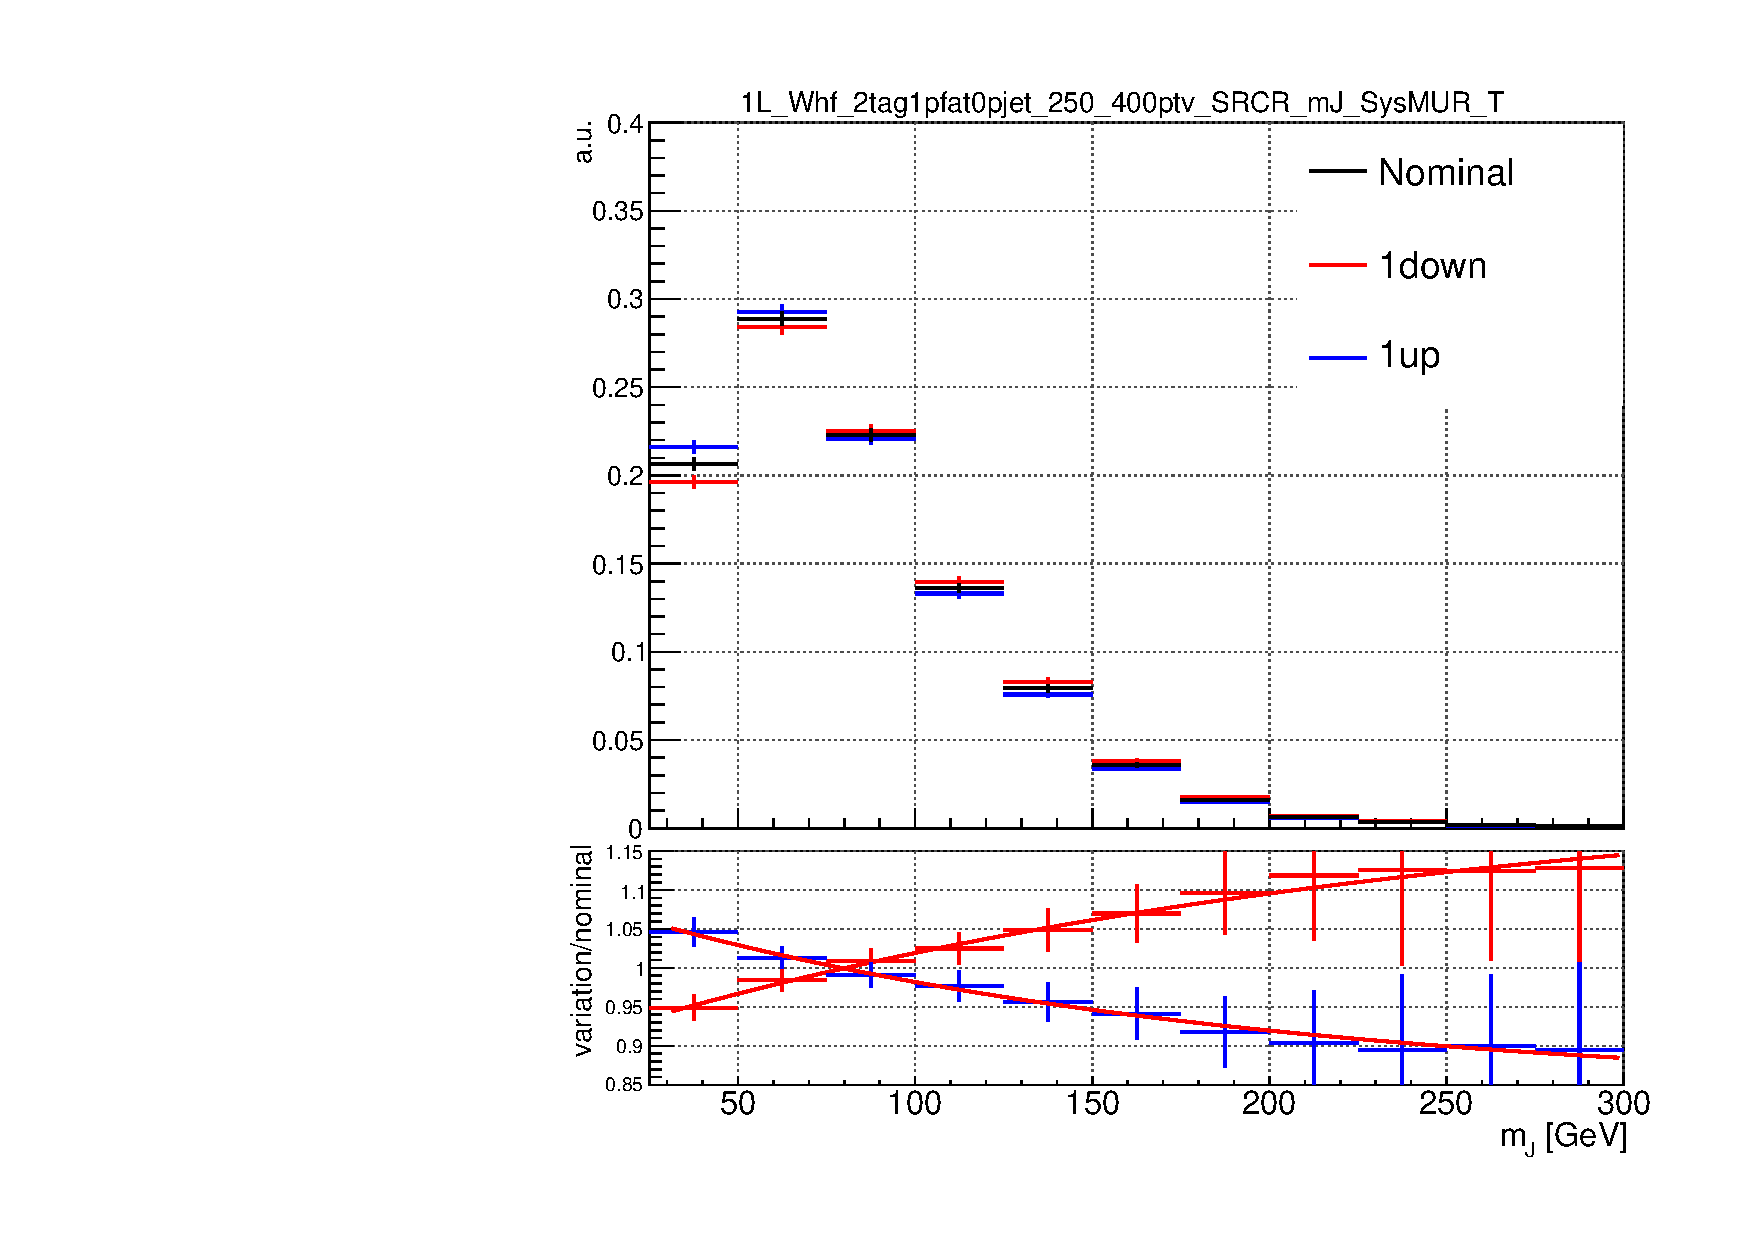
\includegraphics[width=\textwidth]{chapters/6.vhbb_boosted/figs/1L_Whf_2tag1pfat0pjet_250_400ptv_SRCR_mJ_SysMUR_T_Norm.pdf}
      \caption{}
      \label{fig:vhbb muR shape fitted sub1}
    \end{subfigure}%
    \begin{subfigure}{.5\textwidth}
      \centering
      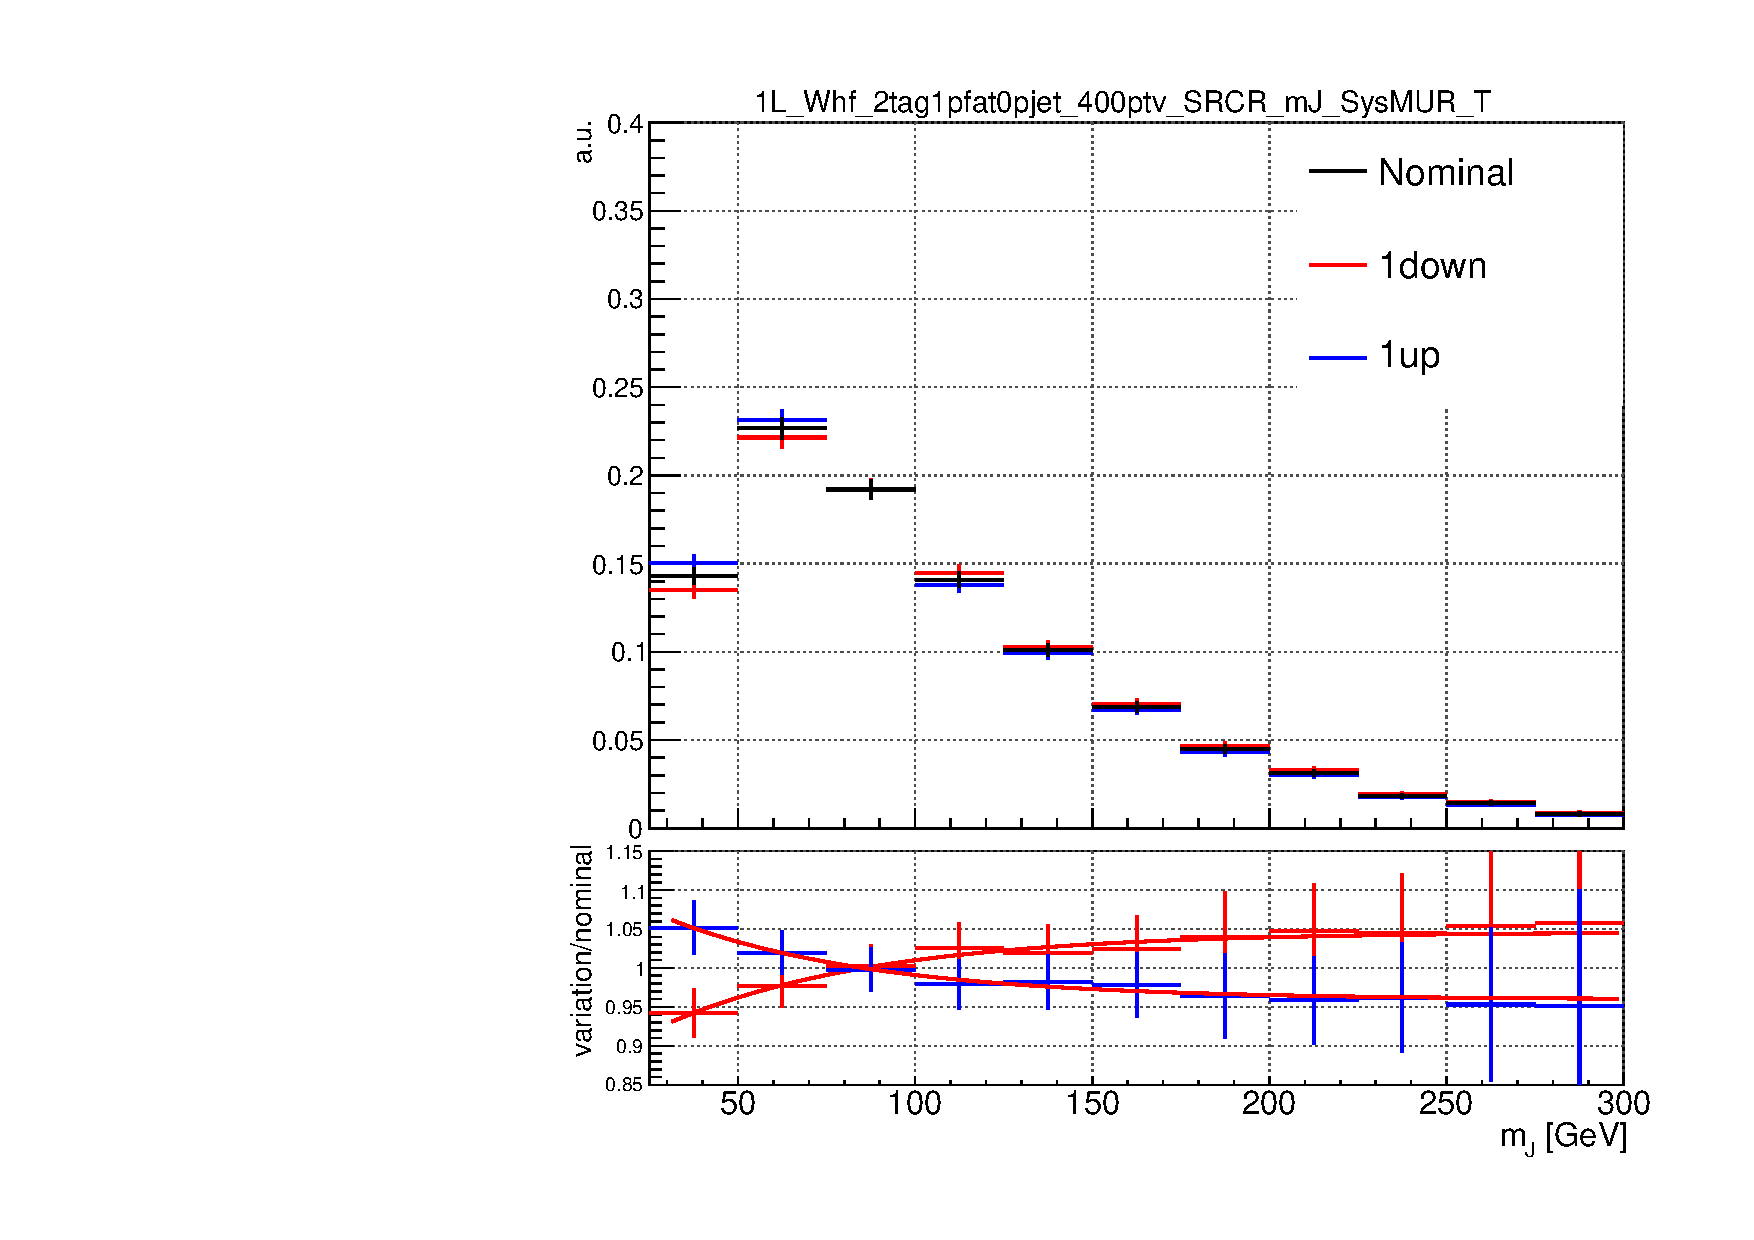
\includegraphics[width=\textwidth]{chapters/6.vhbb_boosted/figs/1L_Whf_2tag1pfat0pjet_400ptv_SRCR_mJ_SysMUR_T_Norm.pdf}
      \caption{}
      \label{fig:vhbb muR shape fitted sub2}
    \end{subfigure}
    \vspace{-0.5em}
    \caption{Normalised distributions of leading fat jet mass $m_J$ for medium (\cref{fig:vhbb muR shape fitted sub1}) and high (\cref{fig:vhbb muR shape fitted sub2}) \pTV analysis regions for W+heavy-flavour-jets (merged in heavy flavours, high and low purity signal regions) in the 0 lepton channel. The renormalisation scale $\mu_R$ has been varied by a factor of 2 (``1up'') and 0.5 (``1down''). An exponential function has been fit to the ratio.}
    \label{fig:vhbb muR shape fitted}
\end{figure}

\subsubsection{Acceptance Uncertainties}
Several different types of acceptance uncertainties have been calculated. These are implemented as nuisance parameters in the fit and for the most part account for the migration of events between different analysis regions. The list acceptance uncertainties relevant to the V+jets processes are given summarised below.
%
\begin{itemize}
    \item \textbf{Overall normalisation:} only relevant where normalisation cannot be left floating (i.e. determined in the fit).
    %
    \item \textbf{SR-to-CR relative acceptance:} the uncertainty on the normalisation of the signal region due to events migrating between the signal and control regions.
    %
    \item \textbf{HP-to-LP relative acceptance:} the uncertainty on the normalisation of the high-purity (HP) signal region due to events migrating between the high- and low-purity signal regions.
    %
    \item \textbf{Medium-to-high} \pTV \textbf{relative acceptance:} describes any 'shape' effect in \pTV distribution, given that the analysis only uses two \pTV bins (medium and high).
    %
    \item \textbf{Flavour relative acceptance:} for each flavour V$xx$, where $xx\in$ \{bc,bl,cc\} the ratio of V$xx$/Vbb events is calculated. This corresponds to the uncertainty of Vbb events due to the miss-tagging of other flavours V$xx$. 
\end{itemize}
%
The uncertainties on different systematics are summed in quadrature to give a total uncertainty on each region. A summary of the different acceptance uncertainties that were derived in this way and subsequently applied in the fit are given in \cref{tab:Vjets acceptance uncerts}. An effort has been made, wherever possible, to harmonise similar uncertainties across different analysis regions and channels.


\subsection{Vector Boson + Jets Modelling}
The background processes involving $W$ or $Z$ boson decays into leptons (including those in which the $W$ boson arises from a top-quark decay) are collectively referred to as electroweak (EW), or V+jets, backgrounds. W+jets events are most relevant to the 1-lepton channel via the leptonic decay of W$\rightarrow \ell\nu$. In the event of W$\rightarrow \tau\nu$, and subsequent decay of the $\tau$, or the lack of the successful reconstruction of the $e$ or $\mu$, W+jets can also contribute to the 0-lepton channel. Meanwhile, Z+jets contributes primarily to the 0- and 2-lepton channels via the processes Z$\rightarrow \nu\nu$ and Z$\rightarrow \ell\ell$ respectively.

Modelling is used to predict the outcomes of the analysis and to assess the impact of sources of different systematic uncertainty. Signal and background modelling has has primarily consisted of using Monte Carlo (MC) generators to produce simulated events. The uncertainties on the simulated output must be well understood to perform a successful analysis. To achieve this, a set of ``nominal'' samples are first defined as a reference to which different variations can be compared. The nominal samples are chosen as the best possible representation of the underlying physical process. ``Alternative'' samples are used to understand the systematic uncertainties on the nominal samples. To generate an alternative sample, some aspect of the model is varied, and the simulation is re-run. A comparison back to the nominal sample gives a handle on the systematic uncertainty associated with the model parameter which was changed. Detailed information can be found in \cite{Bell:2316951}. In order to access uncertainties associated with the use of MC generators, variations of the data are produced using alternative generators or variation of nominal generator parameters. The variation of nominal generator parameters can in certain cases be implemented using internal weight variations stored alongside the nominal events, and in other cases a new independent sample must be generated. The nominal generator used for V+jets events is \textsc{Sherpa 2.2.1}, while \textsc{MadGraph5\_aMC@NLO+Pythia8} (which uses different parton showering models) is used as an alternative generator. As production of large MC samples is computationally expensive, a feature of state of the art simulation packages is to store some sources of variation as internal event weights, which can be generated alongside the nominal samples, saving computation time. Several sources of uncertainty, summarised in \cref{tab:sources of uncertainty}, have been assessed.

%
\begin{table}[!htbp] 
  \footnotesize\centering
  \setlength{\tabcolsep}{0.5em} % for the horizontal padding
  %\def\arraystretch{1.4} 
  \begin{tabular}{l|c|c|c|c}
      \toprule\hline
      \multicolumn{5}{c}{V+jets Acceptance Uncertainties}            
      \\ \hline
      \textbf{Boson}      & \multicolumn{2}{c|}{\textbf{W}} & \multicolumn{2}{c}{\textbf{Z}} 
      \\ \hline
      \textbf{Channel}    & 0L          & 1L         & 0L         & 2L          
      %\\ \hline
      %Vbb Norm.           &   30\%      &     -      &     -      &          -  
      \\ \hline
      SR-to-CR               &   90\%$^\dagger$         & 40\%$^\dagger$ &      40\%     & -         
      \\ \hline
      HP-to-LP SR               & \multicolumn{2}{c|}{18\%}             &   18\%      & -         
      \\ \hline
      Medium-to-high $p_T^V$ &   30\%      & 10\%$^*$       & \multicolumn{2}{c}{10\%}          
      \\ \hline
      Channel relative acceptance             &   20\%      &   -        &    16\%    & -
      \\ \hline
      Vbc/Vbb             & \multicolumn{4}{c}{30\%}                       
      \\ \hline
      Vbl/Vbb             & \multicolumn{4}{c}{30\%}                       
      \\ \hline
      Vcc/Vbb             & \multicolumn{4}{c}{20\%}                       
      \\ \hline
      Vcl Norm.           & \multicolumn{4}{c}{30\%}                       
      \\ \hline
      Vl Norm.            & \multicolumn{4}{c}{30\%}                       
      \\ \hline\bottomrule
  \end{tabular}
  \caption{
    \Vjets acceptance uncertainties \cite{Dao:2688371}.
    \Wjets SR and CR uncertainties marked with a superscript $\dagger$ are correlated.
    The 1L \Wjets medium-to-high \pTV uncertainty marked by $*$ is applied as independent and uncorrelated NPs in both HP and LP signal regions.
    %The 0L \Wjets Wbb Norm uncertainty is only applied when a floating normalisation for Wbb cannot be obtained from the 1L channel.
    %A 30\% uncertainty for \Zbb norm is applied in the 1L channel when a floating normalisation for \Zbb cannot be obtained from the 0L or 2L channels.
  }
  \label{tab:Vjets acceptance uncerts}
\end{table}
%

\subsection{Diboson Modelling}



\section{Fit Studies}

\subsection{Fit Model}
A global profile likelihood fit is used to extract the signal strength $\mu$ and its significance from the data. This statistical setup treats each bin as a Poisson counting experiment. The combined likelihood over $N$ bins, without considering sources of systematic uncertainty, is given by
%
\begin{equation}
    \mathcal{L}(\mu) = \prod_{i=1}^N \frac{(\mu s_i + b_i)^{n_i}}{n_i!} \exp \left[ - (\mu s_i + b_i) \right],
\end{equation}
%
where $s_i$ ($b_i$) is the expected number of signal (background) events in bin $i$, and $n_i$ is the number of events observed in data in bin $i$. The presence of systematic uncertainties which can affect the expected numbers of signal and background events necessitates the addition of nuisance parameters (NPs), $\theta$, to the likelihood. Each source of systematic uncertainty for V+jets samples discussed in the previous section was implemented as a NP $\theta_j$ in the fit. The presence of NPs modifies the likelihood as 
%
\begin{equation}
    \mathcal{L}(\mu) \rightarrow \mathcal{L}(\mu, \theta) = \mathcal{L}(\mu) \times \mathcal{L}(\theta) ~,~~~~ s_i \rightarrow s_i(\theta) ~,~~~~ b_i \rightarrow b_i(\theta),
\end{equation}
%
where
%
\begin{equation}
    \mathcal{L}(\theta) = \prod_{\theta_j \in \theta} \frac{\exp\left[{-\theta_j^2/2}\right]}{\sqrt{2\pi}}.
\end{equation}
%
Post-fit $m_J$ distributions in the high-purity medium \pTV regions for the 0- and 2-lepton channels are shown in \cref{fig:vhbb postfit plots}. The plots show large falling backgrounds, predominantly made up of W+jets and Z+jets events, and a signal distribution corresponding to the Standard Model Higgs boson peaking around $m_H = 125$ GeV.
%
\begin{figure}[!htbp]
    \centering
    \begin{subfigure}{.5\textwidth}
      \centering
      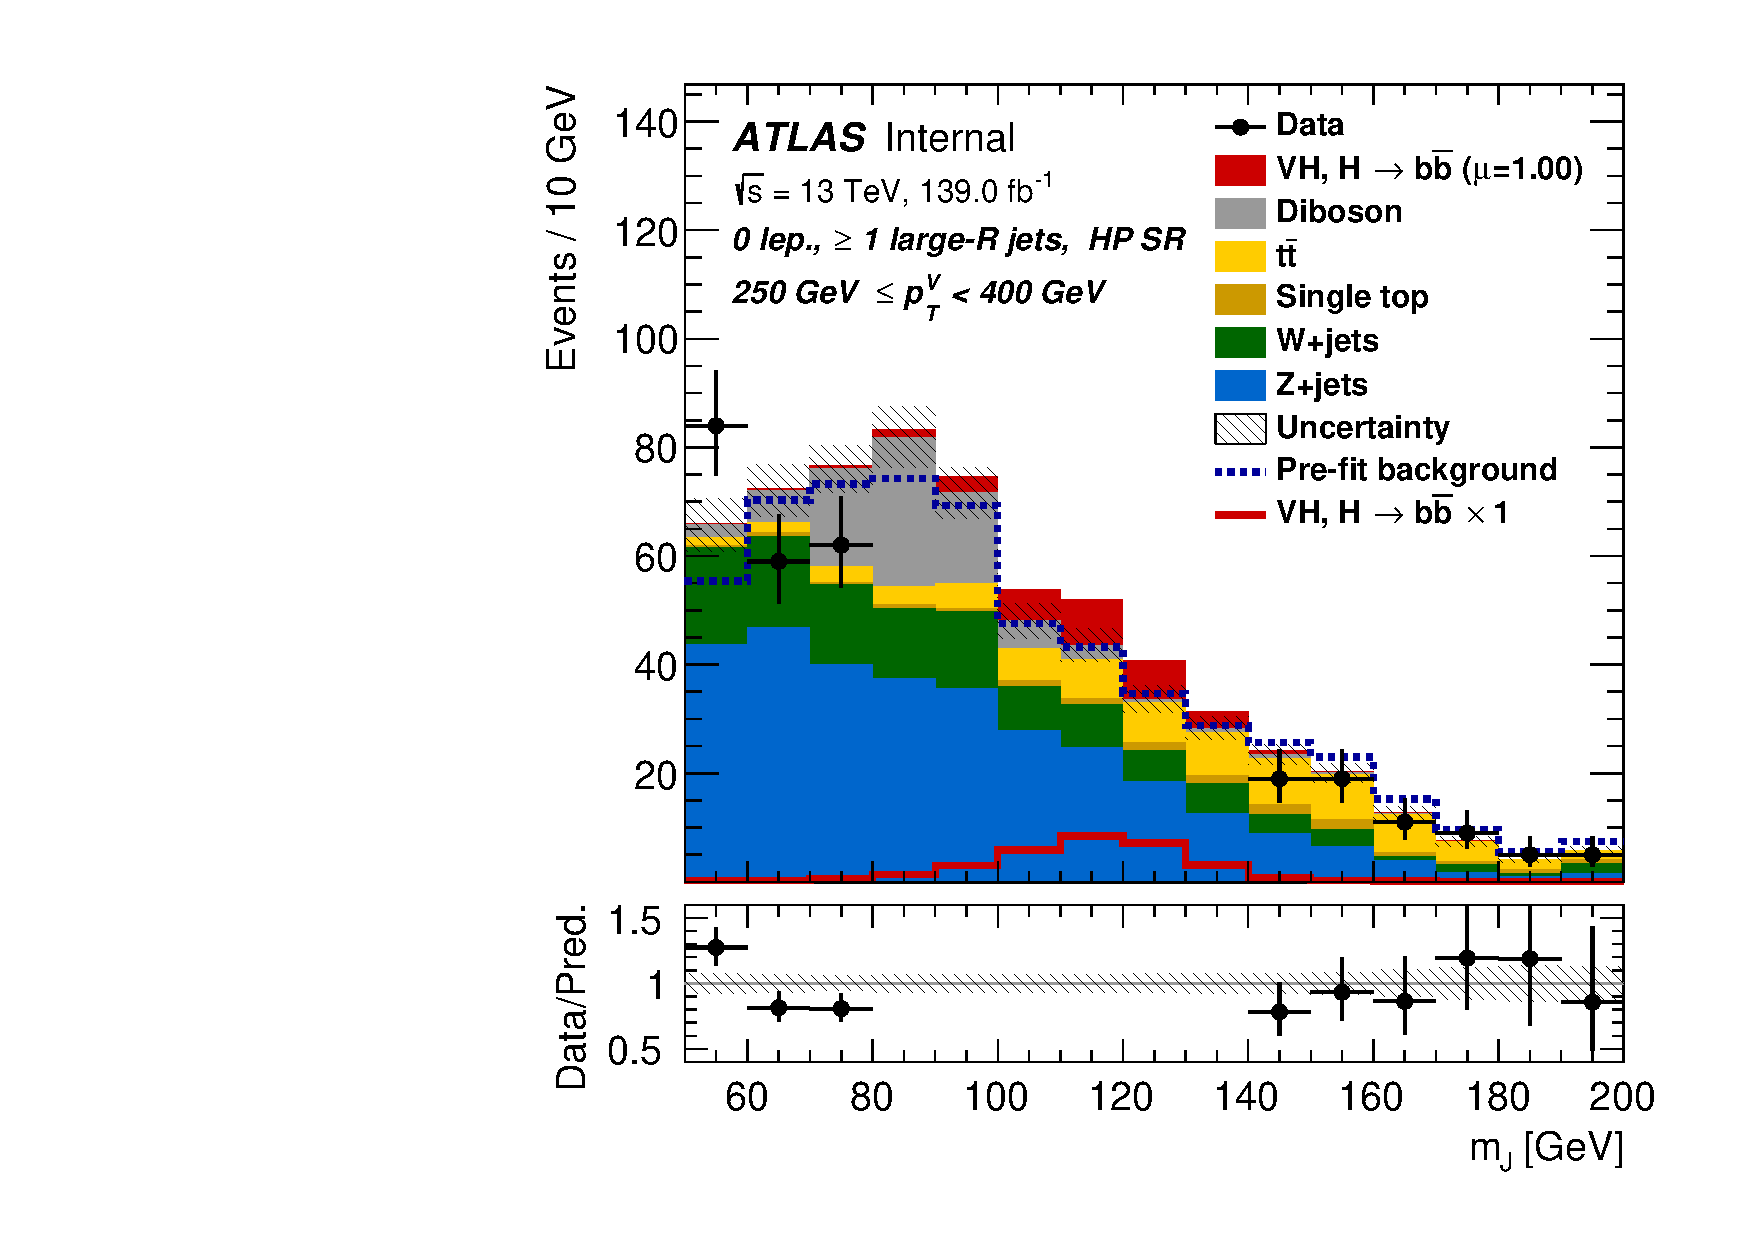
\includegraphics[width=\textwidth]{chapters/6.vhbb_boosted/figs/Region_BMax400_BMin250_incFat1_Fat1_Y6051_DSRnoaddbjetsr_T2_L0_distmBB_J0_GlobalFit_conditionnal_mu1.pdf}
      \caption{}
      \label{fig:vhbb postfit plots sub1}
    \end{subfigure}%
    \begin{subfigure}{.5\textwidth}
      \centering
      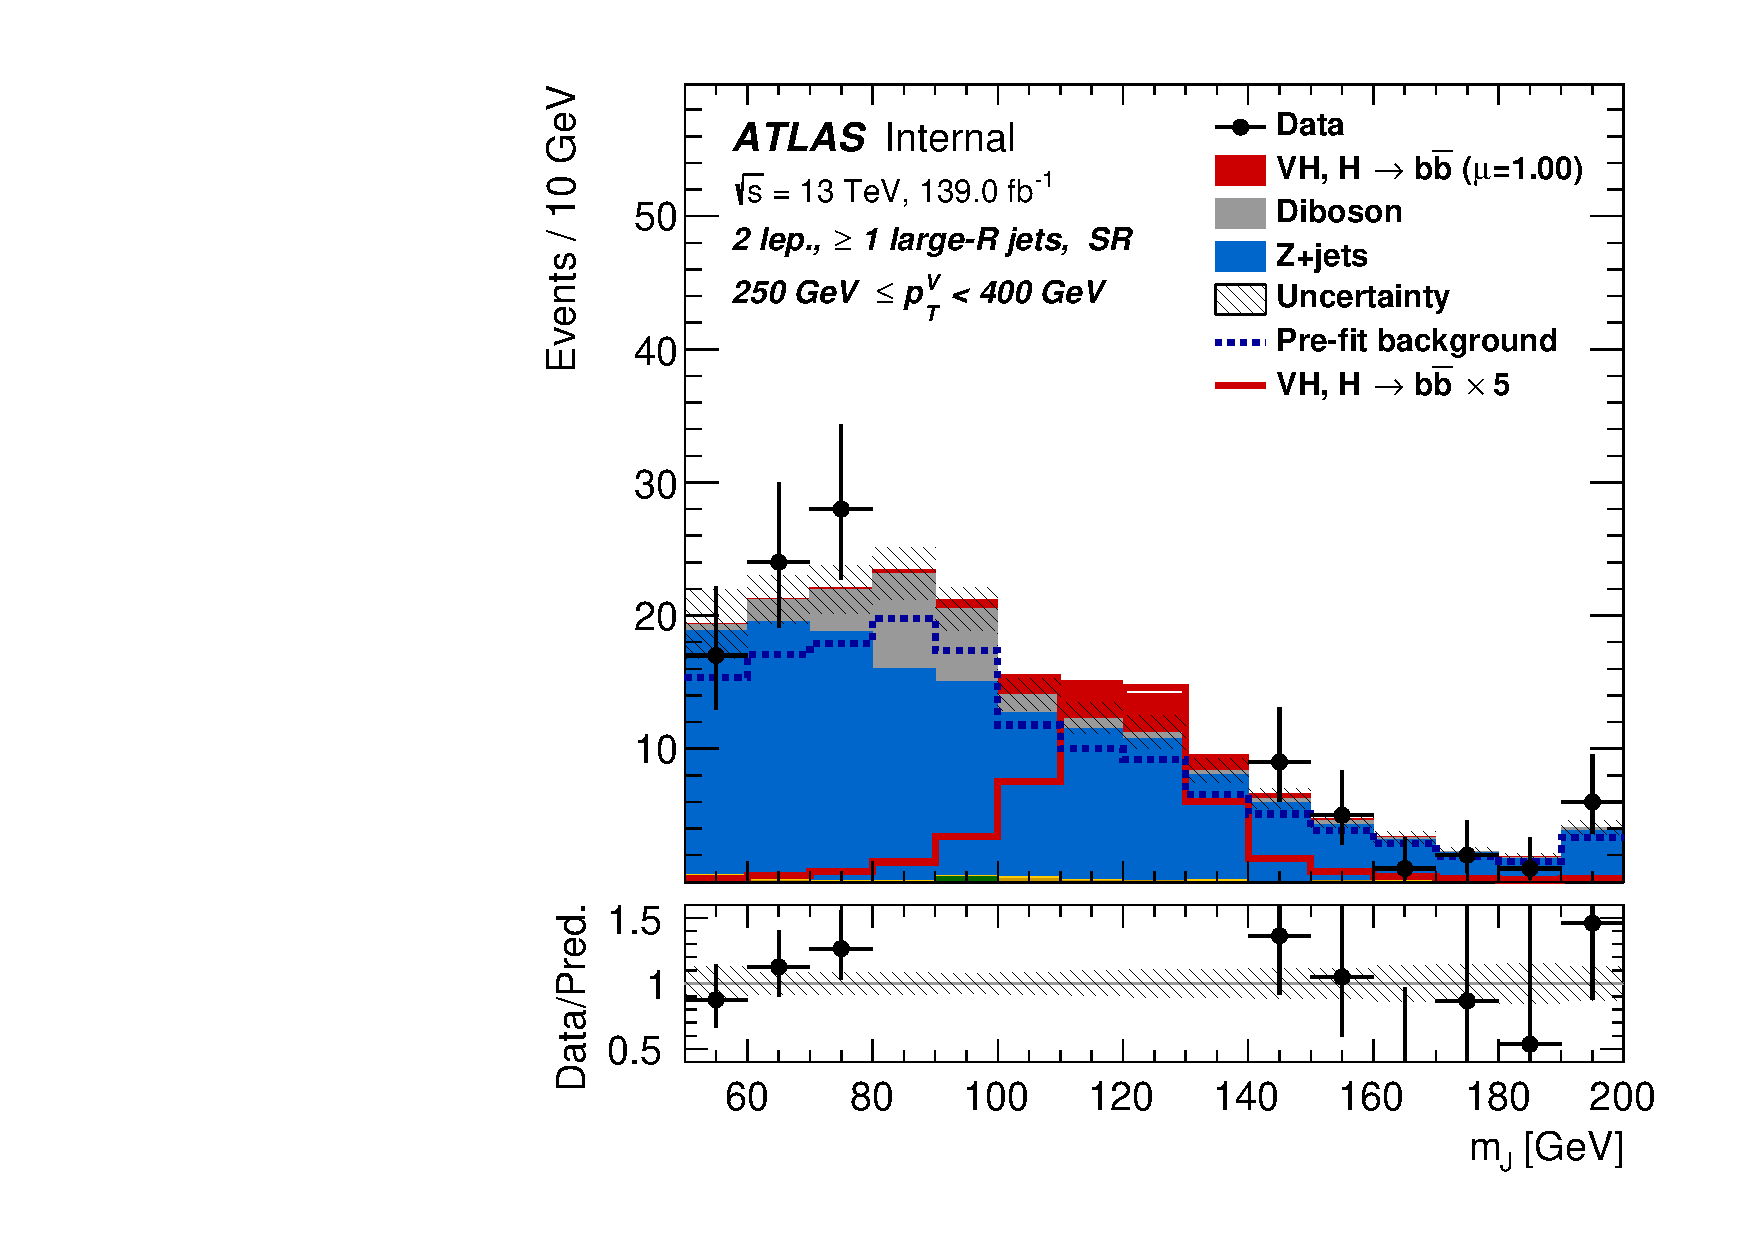
\includegraphics[width=\textwidth]{chapters/6.vhbb_boosted/figs/Region_distmBB_J0_L2_T2_DSR_Y6051_incJet1_Fat1_incFat1_BMin250_BMax400_GlobalFit_conditionnal_mu1.pdf}
      \caption{}
      \label{fig:vhbb postfit plots sub2}
    \end{subfigure}
    \vspace{-0.5em}
    \caption{Post-fit distributions for the 0-lepton (\cref{fig:vhbb postfit plots sub1}) and 2-lepton (\cref{fig:vhbb postfit plots sub2}) channels in the high purity medium \pTV region, obtained in the combined conditional $\mu=1$ fit to data. The last bin of each plot is an overflow bin.}
    \label{fig:vhbb postfit plots}
\end{figure}
%

\section{Conclusion}

Work has been carried out as part of the boosted VHbb analysis group to understand, and implement in the global profile likelihood fit, systematic uncertainties on V+jets samples. This background modelling work is an essential part of the success of the analysis. So far the fit has proved stable with the inclusion of the V+jets uncertainties, and detailed studies are now underway to determine the causes behind any observed pulls of the added NPs. Additional work is ongoing to help with the derivation of uncertainties on diboson samples, another important background. The analysis is already advanced, and is now progressing into its final stages. Publication is expected in the new year.